\chapter{State of the art}
This chapter will give an overview into the background and concepts of this thesis.
In the first section the Internet of Things an related subtopics like Smart Factories and Smart Cities are considered.
Cyber Physical Systems, which are important for the development of Smart Factories are also covered in this section.
Virtualization in general is the main topic of the second section.
First we dive into the area of Virtual Machines, followed by Container Virtualization.
Both are related to each other and sharing some basic ideas.
Container Orchestration as an own subsection show some possibilities of Container Virtualization.
The last subsection Network Function Virtualization concludes with an introduction into the virtualization of network node functions to create communication services.


\section{Internet of Things}
The \ac{IoT} has been a subject of great media- and economically growth in the recent years.
In the year 2008 the number of devices which are connected to the Internet was higher than the human population.\cite[cf.]{Eva11}
Cisco Internet Business Solutions Group predicted that the number will grow up to 50 billion in 2020, this equates to around 6 devices per person.\cite[cf.]{Eva11}
Most of today\'s interactions are \ac{H2H} or \ac{H2M} communication.
The \ac{IoT} on the other hand aim for the \ac{M2M} communication.
This allows every physical devices to be interconnected and to communicate with each other.
These devices are also called "Smart Devices".
Creating a network where all physical objects and people are connected via software is one primary goal of the \ac{IoT}.\cite[cf.]{Rui2015}\cite[cf.]{Kra13}
When objects are able to capture and monitor their environment, a network can perceive external stimuli and respond to them.\cite[cf.][p. 40]{Itu11}
Therefore a new dimension of information and communication technology will be created, where users have access to everything at any time, everywhere.
In addition to smart devices, subcategories are also emerging from the \ac{IoT} which, in addition to the physical devices, also describe technologies such as protocols and infrastructures.
The "`Smart Home"' has been a prominent topic in media and business for many years.
Smart City or Industrie 4.0 are also becoming established and are increasingly popular.
But the Internet started with the appearance of bar codes and \ac{RFID} chips.\cite[cf.]{Kra13}
The second step, which is more or less the current situation, sensors, physical devices, technical devices, data and software are connected to each other.\cite[cf.]{Kra13}
This was achieved, in particular, by cloud computing, which provides the highly efficient memory and computing power that is indispensable for such networks.\cite[cf.]{Rui2015}
The next step could be a "`Cognitive Internet of Things"', which enables easier object and data reuse across application areas, for example through interoperable solutions, high-speed Internet connections and a semantic information distribution.\cite[cf.]{Kra13}
Just as the omnipresent information processing in everyday life, also known as "`Ubiquitous Computing"', which was first mentioned in the "`The Computer for the 21st Century"'\cite[cf.]{Wei91} by Marks Weiser, it will take some time until it is ubiquitous.


\subsection{Industry 4.0 and Smart Factories}

The industry as an changing environment is currently in the state of the so called "fourth industrial revolution".
The first industrial revolution was driven by steam powered machines.
Mass production and division of labor was the primary improvement of the second industrial revolution, whereas the third revolution was characterized by using electronics and the integration of \ac{IT} into manufacturing processes.\cite[cf.][p. 1]{Lom2016}
In the recent years the size, cost and power consumption of chipsets are reduced which made it possible to embed sensors into devices and machines much easier and cheaper.\cite[cf.][p. 1]{Brito2016}
The "Industrie 4.0" is the fourth step in this evolution and was first mentioned at the Hannover Fair in 2011.\cite[cf.][p. 1]{Lom2016}
"Industrie 4.0 is a collective term for technologies and concepts of value chain organization."\cite[cf.][p. 11]{Her2015}

Significantly higher productivity, efficiency, and self-managing production processes where everything from machines up to goods can communicate and cooperate with each other directly are the visions of the Industry 4.0.\cite[cf.]{Lyd2016}
It also aims for an intelligent connection between different companies and units.
Autonomous production and logistics processes creating a real-time lean manufacturing ecosystem that is more efficient and flexible.\cite[cf.]{Lyd2016}
"This will facilitate smart value-creation chains that include all of the life-cycle phases of the product from the initial product idea, development, production, use, and maintenance to recycling."\cite{Lyd2016}
At the end, the system can use customer wishes in every step in the process to be flexible and responsive.\cite[cf.]{Lyd2016}

\begin{table}[htpb]
  \centering
  \begin{tabular}{| r | c c c c |}
  	\rowcolor{dunkelgrau}
  	\hline
  	                      & Cyber-Physical & Internet  & Internet    & Smart Factory \\
    \rowcolor{dunkelgrau}
                          & Systems        & of Things & of Services &  \\
  	\hline
  	Interoperability      & X        & X        & X          & X    \\
  	Virtualization        & X        & -        & -          & X    \\
    Decentralization      & X        & -        & -          & X    \\
    Real-Time Capability  & -        & -        & -          & X    \\
    Service Orientation   & -        & -        & X          & -    \\
    Modularity            & -        & -        & X          & -    \\
  	\hline
  \end{tabular}
  \caption[Design principles of each Industry 4.0 component]{Design principles of each Industry 4.0 component.\cite[cf.][p. 11]{Her2015}}
  \label{tab:industryComponents}
\end{table}

Table \ref{tab:industryComponents} shows the six design principles which can be from the Industrie 4.0 components.
They can help companies to identify and implement Industry 4.0 scenarios.\cite[cf.][p. 11]{Her2015}

\begin{enumerate}
  \item \textit{Interoperability} \ac{CPS} of various manufacturers are connected with each other. Standards will be the key success factor in this area.\cite[cf.][p. 11]{Her2015}
  \item \textit{Virtualization} \ac{CPS} are able to monitor physical processes via sensors. The resulting data is linked to virtual plant and simulation models. These models are virtual copies of physical world entities.\cite[cf.][p. 11]{Her2015}
  \item \textit{Decentralization} \ac{CPS} are able to make decisions on their own, for example when \ac{RFID} chips send the necessary working steps to the machine. Only in cases of failure the systems delegate task to a higher level.\cite[cf.][p. 11]{Her2015}
  \item \textit{Real-Time Capability} Data has to be collected and analyzed in real time and the status of the plant is permanently tracked and analyzed. This enables the \ac{CPS} to react to a failure of a machine and can reroute the products to another machine.\cite[cf.][p. 11]{Her2015}
  \item \textit{Service Orientation} \ac{CPS} are available over the \ac{IoS} and can be offered both internally and across company borders to different participants. The manufacturing process can be composed based on specific customer requirements.\cite[cf.][p. 11]{Her2015}
  \item \textit{Modularity} The system is able to be adjusted in case of seasonal fluctuations or changed product characteristics, by replacing or expanding individual modules.\cite[cf.][p. 11]{Her2015}
\end{enumerate}

Another important aspect of Industry 4.0 is the implementation of process automation with the focused on three distinct aspects.
Starting with the vertical integration, which contains the connection and communication of subsystems within the factory enables flexible and adaptable manufacturing systems.\cite[cf.][p. 7 ff.]{Vbw2014}
The horizontal integration, as the second aspect, enables technical processes to be integrated in cross-company business processes and to be synchronized in real time through multiple participants to optimize value chain outputs.\cite[cf.][p. 7 ff.]{Vbw2014}
Finally end-to-end engineering, planning, and process control for each step in the production process.\cite[cf.]{Lyd2016}

\begin{figure}
    \centering
    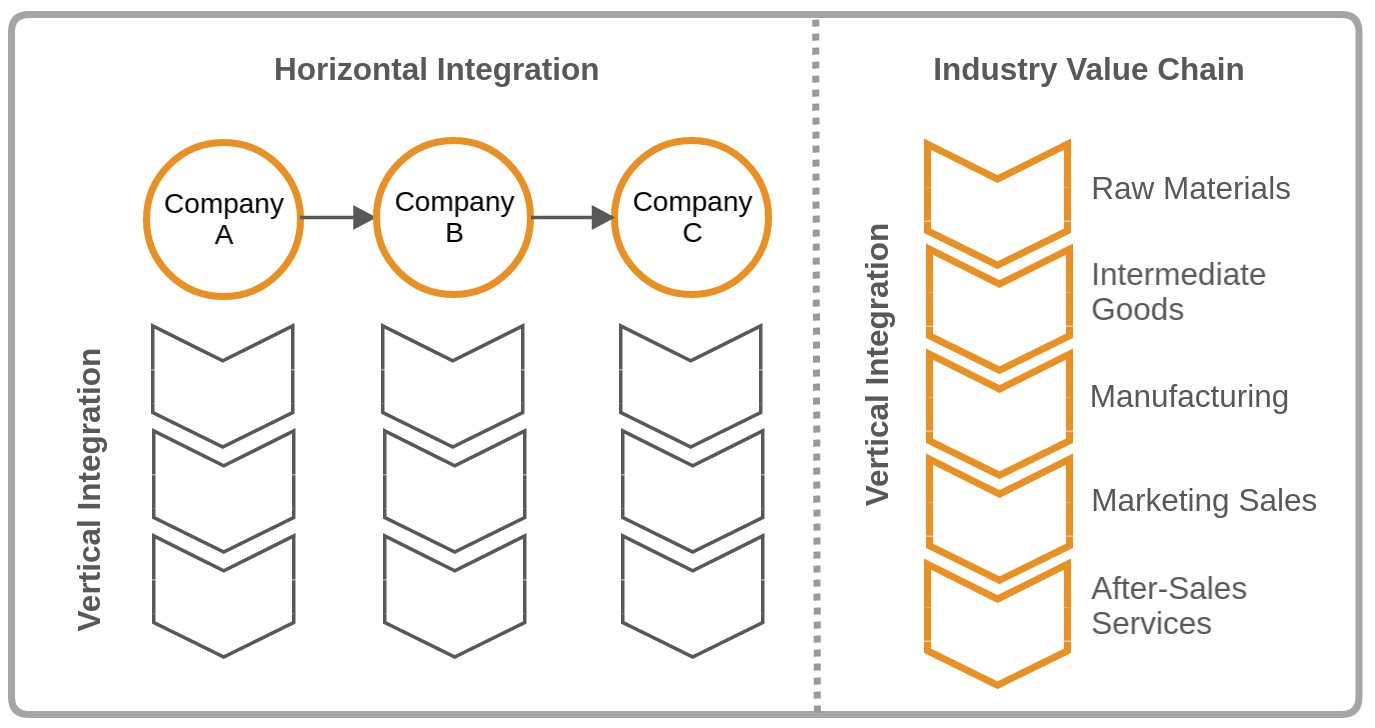
\includegraphics[width=\textwidth]{resources/images/vertical_horizontal_integration.png}
    \caption[Horizontal vs. Vertical Integration]{Horizontal vs. Vertical Integration. Adapted from: \cite{Jur2013}}
    \label{fig:vertical_horizontal_integration}
\end{figure}

Figure \ref{fig:vertical_horizontal_integration} illustrates this concept.
The left side shows the whole production process over company boundaries on the horizontal scale, as well as the industry value chain on the vertical scale which is specific for each company.
On the right side there is an exemplary industry value chain which starts with the raw materials and ends with the sale of the product to illustrates an more specific example of the vertical integration.

\todo{guter abschluss -> moving production steps to each machine -> modular, without core system, locally in the modules -> communication path growth shorter -> self organisation -> decentralized}

\todo{as well as highly flexible, individualized and resource friendly mass production}

% Gute Quelle:
% http://winfwiki.wi-fom.de/index.php/Wertsch%C3%B6pfungsnetzwerke_und_Industrie_4.0

% Masterarbeit Alex
% https://www.yumpu.com/de/document/view/21142108/schriftliche-ausarbeitung-alexander-willner-masterarbeit/5


\subsection{Cyber Physical Systems}

As we already now, in smart factories every physical device is connected to each other.
Everything can be captured and monitored in each step of a production process.
With \acp{CPS} every physical entity has a digital representation in the virtual system.\cite[cf.][p. 1363]{Poovendran2010}
Before a \ac{CS} was passive, which means it has no communication between the physical and the virtual world.\cite[cf.][p. 1364]{Poovendran2010}
While new technologies in the physical world, like new materials, hardware and energy, are developed, the technologies in the virtual worlds are also being improved, for example through the use of new protocols, networking, storage and computing technologies.\cite[cf.][p. 1364]{Poovendran2010}
This adds more intelligence in such systems, as well as a much more flexible and modular structure.
A \ac{CPS} can organize production automatically and autonomously, which eliminate the need of having a central process control.\cite[cf.]{Lom}
Thereby the system can handle lossy signals and short range radio technologies, which are widely used in such a context.\cite[cf.]{Yannuzzi2014}
\todo{write more}


\subsection{Fog Computing}
% definition
% probleme taxonomy
% unterschiede
% -- architektur
% abgrenzung


\section{Virtualization}
According to the \ac{NIST} the definition of virtualization is: "Virtualization is the simulation of the software and/or hardware upon which other software runs. This
simulated environment is called a virtual machine (VM)."\cite{Sca2011}.
This means a \ac{VM}, also referred as guest system, can be executed in a real system, which is referred as host system.
Basically there are two types of virtualization: Process virtualization where the virtualizing software also known as \ac{VMM} is executed by the host \ac{OS} and only an application will be executed inside the guest \ac{OS} and on the other side there is the the system virtualization where the whole \ac{OS} as well as the application are running inside the virtualizing software.
Figure \ref{fig:vertical_horizontal_integration} illustrate both concepts.
\todo{right figure}
Examples for process virtualization could be the Java Virtual Machine, the .Net framework or Docker, where VMWare, Oracle Virtual Box, XEN or Microsoft Hyper-V are only some examples for system virtualization.
\todo{footnotes or bibs?}
The benefits of all virtualization techniques are the rapid provisioning of resources which could be \ac{RAM}, disk storage, computation power or network bandwidth.
Beside that, no human interaction is necessary during the provisioning process.
Elasticity which scales a system in a cost-efficient manner in both directions, up and down.
Customer as well as the provider profit from such a system.
Security based on the isolation of the \acp{VM} is another huge benefit.
Different processes can not interfere with each other and the data of a single user can not be accessed by other users of the same hardware.
A challenge despite all the mentioned benefits is the performance.
Running \acp{VM} increases the overhead and reduces the overall performance of a system.
Therefore the specific use case have to consider these behavior.


\subsection{Virtual Machines}
\acp{VM} are the core virtualization mechanism in cloud computing.
There are also two different designs for hardware virtualization.
The first and more popular type for cloud computing is the \textit{bare-metal virtualization}.
It needs only a basic OS to schedule \acp{VM}.
The hypervisor runs directly on the hardware of the machine.
This is more efficient, but requires special device drivers to be executed.
The other type is the \textit{hosted virtualization}.
Unlike the first type the \ac{VMM} run as a host \ac{OS} process and the \acp{VM} as a process supported by the \ac{VMM}.
No special drivers are needed for these type of virtualization, but by comparison the overhead is much bigger.
For both types, the performance limitation remains.
Each \ac{VM} need a full guest \ac{OS} image in addition to binaries and libraries which are necessary for the application to be executed.\cite[cf.][p. 381]{Pahl2015}
If only a single application should be executed which only need some binaries and libraries, these virtualization method is too bloated.


\subsection{Container Virtualization}
Container virtualization which is also known as System-level virtualization, is the second virtualization machanism.
It based on fast and lightwight process virtualization to encapsulate an entire application with its dependencies into a ready-to-deploy virtual container.\cite[cf.][p. 72]{Tosatto:2015}

a.\cite{Celesti:2016}
b.\cite{Anderson:2016}


\subsubsection{Linux Containers}
a.\cite{Soltesz:2007}

\subsubsection{Docker}

\todo{"First, we must know what exactly Docker is and does. Docker is a container management system that helps easily manage Linux Container (LXC) in an easier and universal fashion. This lets you create images in virtual environment ons your laptop and run commands or operations against them. The actions you do to the containers that you run in these environments locally on your own machine will be the same commands or operations you run against them when they are running in your production environment. This helps in not having to do things differently when you go from a development environment like that on your local machine to  a production environment like that on your local machine to a production environment on your server. Now, let's take a look at the differences between Docker containers and the typical virtual machine environments.

In the following illustration, we can see the typical Docker setup on the right-hand side versus the typical VM setup on the left-hand side:}
\begin{figure}
    \centering
    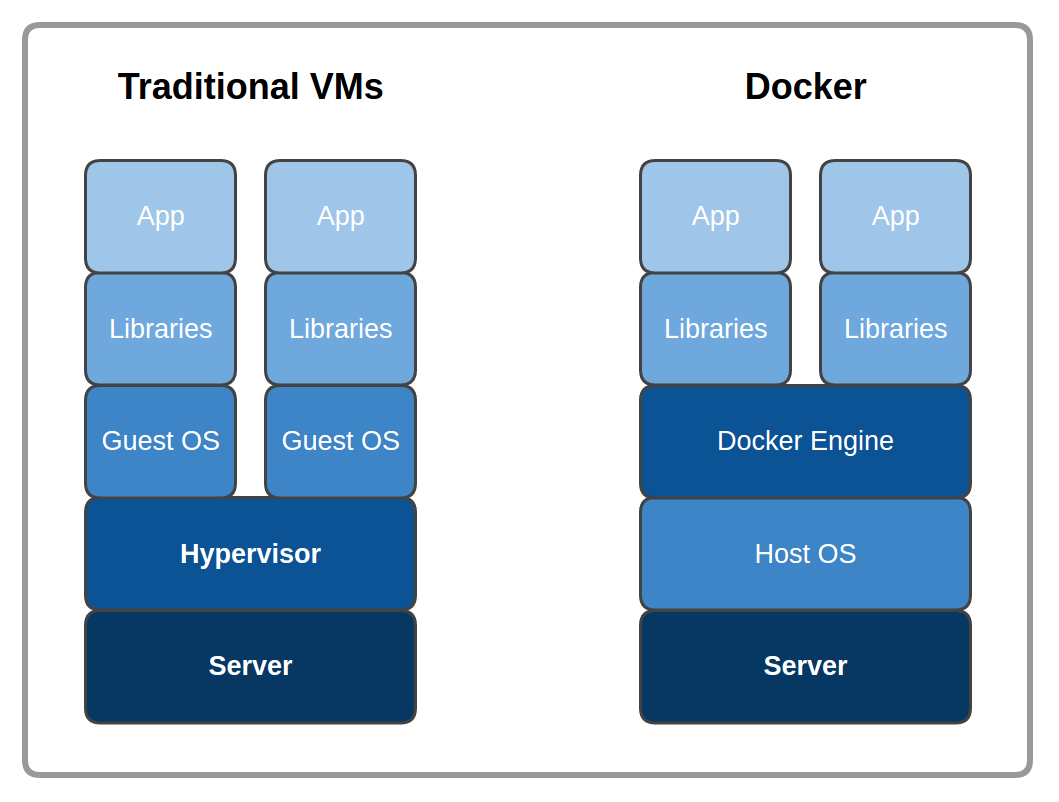
\includegraphics[width=0.6\textwidth]{resources/images/docker_vs_vm.png}
    \caption[Structure traditional VMs vs. Docker]{Structure traditional VMs vs. Docker. Adapted from: \cite[p. 2]{Gal2015}}
    \label{fig:vms_vs_docker}
\end{figure}

\todo{"This illustration gives us a lot of insight into the biggest key benefit of Docker, that is, there is no need for a complete operating system every time we need to bring up a new container, which cuts down on the overall size of containers. Docker relies on using the host OS's Linux kernel (since almost all the versions of Linux use the standard kernel models) for he OS it was build upon, such as Red Hat, CentOS, Ubuntu, and so on. For this reason, you can have almost any Linux OS as your host operating system (Ubuntu in the previous illustration) and be able to layer other OSes on top of the host. For example, in the earlier illustration, we could have Red Hat running for one app (the one on the left) and Debian running for the other app (the one on the right), but there would never be need to actually install Red Hat or Debian on the host. Thus, another benefit of Docker is the size of an images when they are born. They are not build with the largest piece: the kernel or the operating system. This makes them incredibly small, compact, and easy to ship."\cite{Gal2015}}


\subsection{Container Orchestration}

\subsubsection{Kubernetes}

\subsubsection{Docker Swarm}


\subsection{Network Function Virtualization}


\section{Conclusion}
